% Appendix A
\section{XBee join and send time experiments} % Main appendix title
\label{AppendixA} 
\subsection{Distance relation test}
This table contains the results of two different test programs (blue and green values). The program scenario is as follows:\\
\begin{enumerate}
\item Turn on Waspmote and XBee from \textit{Hibernate}
\item Wait until XBee has joined (Reduced setup mode)
\item Measure battery level, temperature, humidity and pressure (each with 100 milliseconds delay between samples)
\item Send the values and turn off Waspmote (enable \textit{Hibernate})
\vspace{1cm}
\end{enumerate} 
\vspace{1cm}
\noindent
We can conclude that the join time remains constant but the send time and energy consumption increase when more obstacles must be overcome.
\begin{figure}[htbp]
\centering
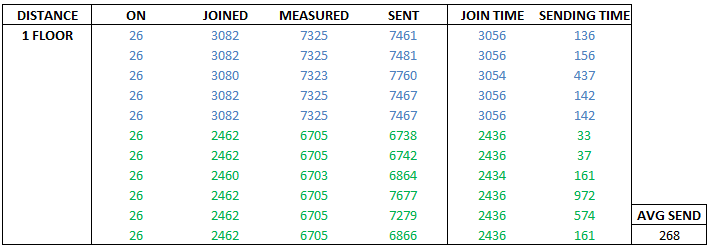
\includegraphics[height=5.5cm]{floors1}
\caption[XBee join and send times: distance relation]{Measurements of join and send time at different distances.}
\label{fig:floors1}
\end{figure}
\begin{figure}[htbp]
\centering
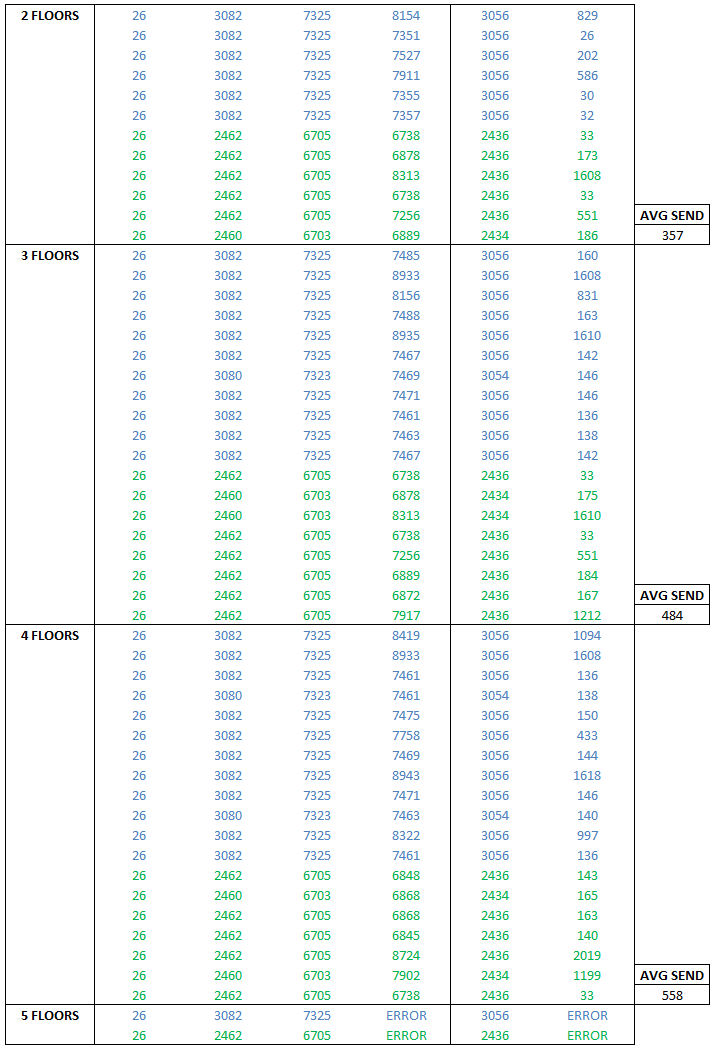
\includegraphics[height=23cm]{floors2}
\caption[XBee join and send times: distance relation]{Measurements of join and send time at different distances}
\label{fig:floors2}
\end{figure}

\pagebreak
\subsection{First time reduction}

The next results are obtained via the following scenario:\\

\begin{enumerate}
\item Turn on Waspmote and XBee
\item Measure battery level, temperature, humidity and pressure (each with 100 milliseconds delay between samples)
\item Check XBee association (Reduced setup mode)
\item Send the values and turn off Waspmote
\end{enumerate}
\vspace{1cm}
\noindent
It appears that when the XBee has been on for a sufficient amount of time, the time to request the node's association state is constant at about 450ms.\\
A second conclusion is that without obstacles and with a node that already is joined a while before trying to send leads to a constant sending time.\\  \bigskip \bigskip
\hspace{5cm}
\begin{figure}[htbp]
\centering
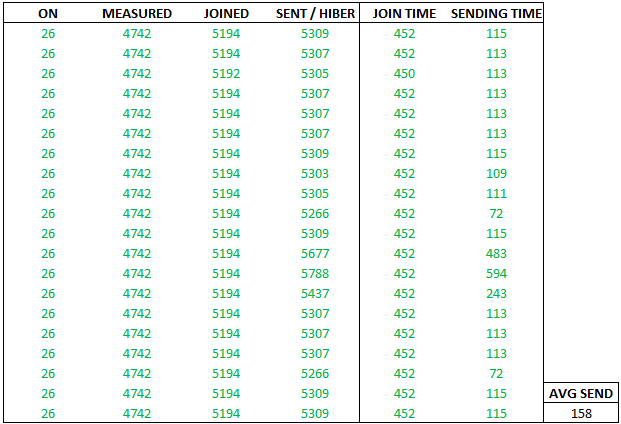
\includegraphics[height=10.5cm]{floors3}
%\rule{30em}{0.5pt}
\caption[XBee join and send times: first time reduction]{XBee join and send times: first time reduction}
\label{fig:floors3}
\end{figure}
\vfill
\pagebreak
%------------------------------------------------------------------
\subsection{Second time reduction}
\label{second}
The next results are obtained via the following scenario:\\

\begin{enumerate}
\item Turn on Waspmote and XBee
\item Measure battery level, temperature, humidity and pressure (without delay between samples)
\item Check XBee association (Reduced setup mode)
\item Send the values and turn off Waspmote
\end{enumerate}
\vspace{1cm}
\noindent
The sensors are measured after 708ms. However it takes about 2.5 seconds for the XBee to join the network. The total average time the Waspmote is turned on is 3 seconds.
\begin{figure}[htbp]
\centering
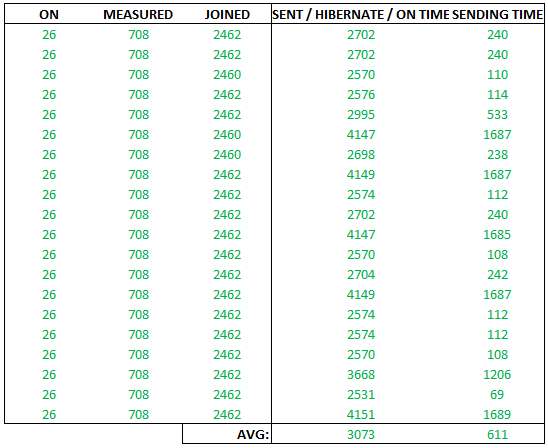
\includegraphics[height=10.5cm]{joinTimes}
\caption[XBee join and send times: second time reduction]{XBee join and send times: second time reduction}
\label{fig:joinTimes}
\end{figure} 
\vfill
\pagebreak
%------------------------------------------------------------------
\subsection{Sensor measuring experiments}
\label{sensMeasuring}
\subsubsection{Temperature measurements with and without delay between the readings}
\begin{table}[!hb]
\begin{center}
\begin{tabular}[!hb]{|c|c|}
\hline
Typical consumption  & 6 $\mu$A\\
\hline
Time needed with delay & 1050ms\\
\hline
Time needed without delay & 47ms\\
\hline
\end{tabular}
%\caption{Individual Sensor Sleep Times in seconds}
\label{tab:sleep1}
\end{center}
\end{table}
\begin{figure}[htbp]
\centering
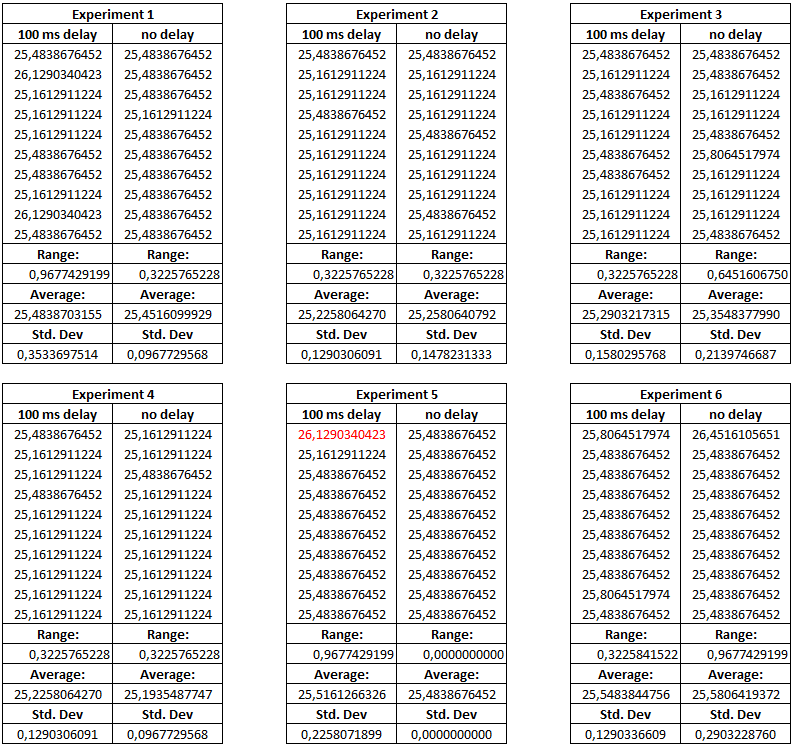
\includegraphics[height=15cm]{temperatures}
\caption{Temperature measurements with and without delay between the readings}
\label{fig:temperatures}
\end{figure} 
\vfill
\pagebreak
%----------------------
\subsubsection{Humidity measurements with and without delay between the readings}
\begin{table}[!hb]
\begin{center}
\begin{tabular}[!hb]{|c|c|}
\hline
Typical consumption  & 0.38mA\\
\hline
Time needed with delay & 1049ms\\
\hline
Time needed without delay & 48ms\\
\hline
\end{tabular}
%\caption{Individual Sensor Sleep Times in seconds}
\label{tab:sleep1}
\end{center}
\end{table}
\begin{figure}[htbp]
\centering
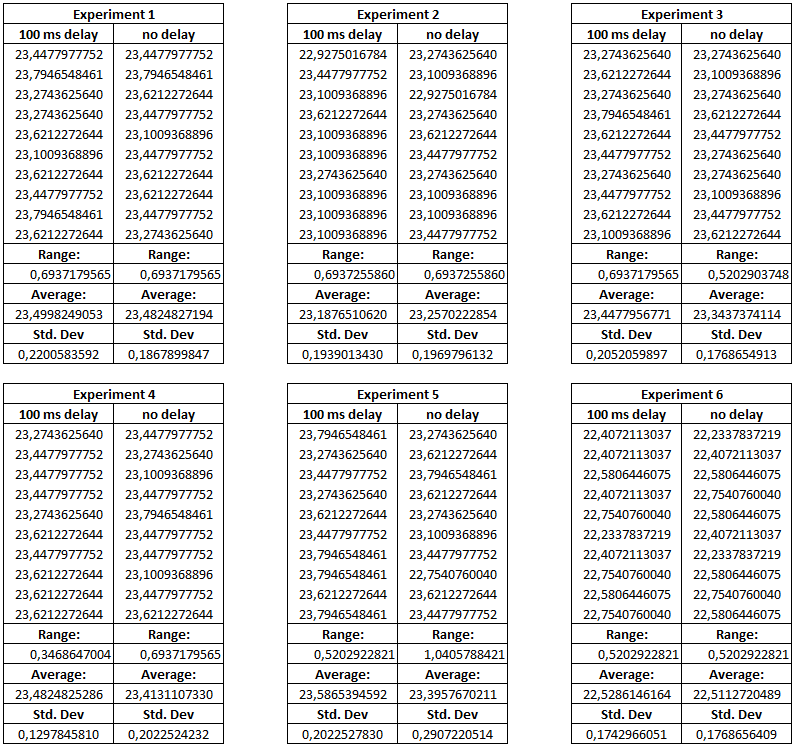
\includegraphics[height=15cm]{humidities}
\caption{Humidity measurements with and without delay between the readings}
\label{fig:humidities}
\end{figure} 
%------------------------------
\vfill
\pagebreak
\subsubsection{Pressure measurements with and without delay between the readings}
\begin{table}[!hb]
\begin{center}
\begin{tabular}[!hb]{|c|c|}
\hline
Typical consumption  & 0.7mA\\
\hline
Time needed with delay & 1053ms\\
\hline
Time needed without delay & 51ms\\
\hline
\end{tabular}
%\caption{Individual Sensor Sleep Times in seconds}
\label{tab:sleep1}
\end{center}
\end{table}
\begin{figure}[htbp]
\centering
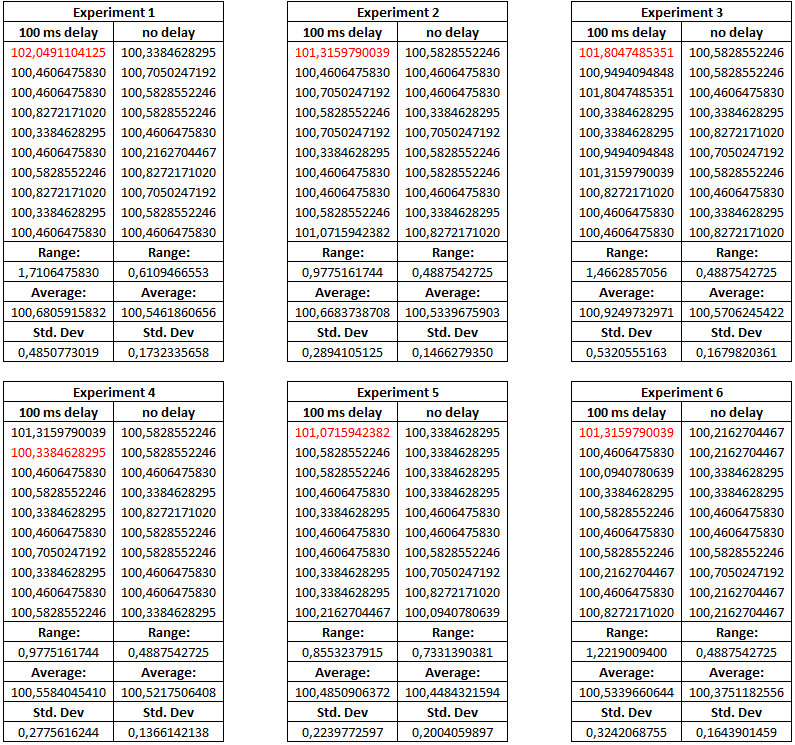
\includegraphics[height=15cm]{pressures}
\caption{Pressure measurements with and without delay between the readings}
\label{fig:pressures}
\end{figure} 
\vfill
\pagebreak
%----------------------
\subsubsection{Pressure measurements with and without delay between the readings}
\begin{table}[!hb]
\begin{center}
\begin{tabular}[!hb]{|c|c|}
\hline
Time needed with delay & 1014ms\\
\hline
Time needed without delay & 11ms\\
\hline
\end{tabular}
%\caption{Individual Sensor Sleep Times in seconds}
\label{tab:sleep1}
\end{center}
\end{table}
\begin{figure}[htbp]
\centering
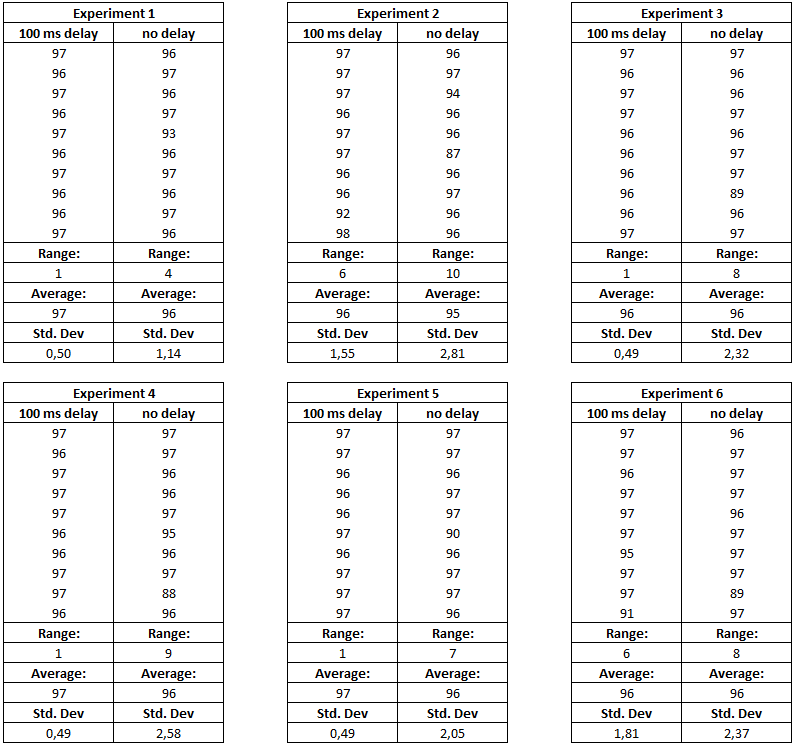
\includegraphics[height=15cm]{batteries}
\caption{Battery measurements with and without delay between the readings}
\label{fig:batteries}
\end{figure} 